\documentclass[11pt]{article}

% --- packages ---------------------------------------------------------------
\usepackage[a4paper,margin=1in]{geometry}
\usepackage{lmodern}
\usepackage[T1]{fontenc}
\usepackage[utf8]{inputenc}
\usepackage{microtype}
\usepackage{graphicx}
\usepackage{booktabs}
\usepackage{siunitx}
\usepackage{xcolor}
\usepackage{caption}
\usepackage{amsmath}
\usepackage[colorlinks=true,allcolors=black,urlcolor=blue!55!black]{hyperref}

\graphicspath{{../figures/}}

% --- style ------------------------------------------------------------------
\definecolor{ink}{HTML}{1A1A1A}
\definecolor{muted}{HTML}{6A6A6A}
\color{ink}
\captionsetup{font=small,labelfont=bf,labelsep=period}
\sisetup{group-separator={,},group-minimum-digits=4,detect-weight=true}
\setlength{\parskip}{0.35em}
\setlength{\parindent}{0pt}
\renewcommand{\arraystretch}{1.15}

% headline number macro
\newcommand{\headline}[1]{\textbf{#1}}

\title{\vspace{-1.5em}\textbf{\Large ZOMBI2 performance}\\[0.3em]
  \large Scaling of species-tree and gene-family simulation}
\author{Performance analysis\\ \small\color{muted} generated for the ZOMBI2 project}
\date{\small 2026-07-04}

\begin{document}
\maketitle
\vspace{-1.5em}

% --- abstract ---------------------------------------------------------------
\begin{abstract}
\noindent
We benchmark the two core operations of ZOMBI2 --- simulating a species tree and
evolving gene families along it --- across five orders of magnitude in tree size, on
a single laptop, and set them against the legacy ZOMBI~1. Both operations are
essentially linear in the number of tips: a \headline{three-million-tip species tree}
is simulated in \headline{$\approx$18\,s using $\approx$2\,GB}, and
\headline{one-million-tip} gene-family copy-number profiles in
\headline{$\approx$18\,s using $\approx$3.2\,GB}. Gene families are emitted in one of
three modes --- a full per-event log, a compact \emph{event trace} (from which gene
trees stay reconstructable), and a counts-only profile. The trace and profile paths
scale to a million tips, whereas the full log tops out near \num{100000} because it
materialises one Python object per event. The dense
$\text{families}\times\text{species}$ profile matrix, quadratic in tip count, was the
one component that did not scale; a sparse (COO) representation moved its ceiling from
$\sim$\num{100000} to several million. Replicate-level parallelism gives a
$3.9\times$ speed-up on a 10-core chip. On the identical gene-family task, ZOMBI2 runs
\headline{over $1000\times$ faster than ZOMBI~1} and keeps scaling far past ZOMBI~1's
$\sim$\num{1200}-tip practical ceiling. All raw timings, the code that produced them,
and these figures are reproducible from the \texttt{performance\_analysis/} workspace.
\end{abstract}

% --- setup ------------------------------------------------------------------
\section{Setup and methodology}

\textbf{Workload.} Every benchmark uses one fixed regime so the numbers stay
comparable: a birth--death species model $\text{BirthDeath}(\lambda{=}1.0,\,
\mu{=}0.3)$ of crown age $2.0$, and gene families evolving under uniform per-copy
rates ($D{=}0.2$, $T{=}0.1$, $L{=}0.25$, $O{=}0.5$; \num{20} founding families).
Loss exceeds duplication, so family sizes never run away. The built-in model runs
on the compiled \texttt{zombi2\_core} (Rust) engine, which \texttt{simulate\_genomes}
selects automatically.

\textbf{Measurement.} Wall-clock time is taken with a monotonic clock
(\texttt{time.perf\_counter}) after one untimed warm-up; each point is repeated
several times and we report the \emph{median} with a shaded inter-quartile
(25--75\%) band. Each timed repeat runs with the cyclic garbage collector
\emph{disabled} (with a full \texttt{gc.collect()} between repeats), exactly as
\texttt{timeit} does: without this the object-heavy full-log path swings wildly as a
collection fires at a different point each run: this isolates intrinsic cost from the
collector's schedule. Species trees are built once per size and reused across the
gene-family series, so those comparisons are a fair A/B on identical inputs; only the
timed call sits inside the timer. Peak memory (resident set size) is measured in an
\emph{isolated subprocess} per size --- the only way to get a clean per-size figure
from a high-water-mark counter --- and there the collector is left \emph{on}, so the
memory numbers reflect a normal run.

\textbf{Machine.} Apple Silicon, 10 cores (4 performance + 6 efficiency), 34\,GB
RAM, macOS; CPython 3.12, ZOMBI2 \texttt{0.2.0.dev0}. Absolute numbers are
machine-specific; the \emph{scaling} is not.

% --- species tree -----------------------------------------------------------
\section{Species-tree simulation scales to millions of tips}

Simulating the species tree is $O(N)$ in the number of tips and featherweight
(Figure~\ref{fig:tree}). The backward reconstructed sampler --- the default, which
conditions on $N$ extant tips --- takes \SI{50}{\milli\second} at \num{10000} tips,
\SI{0.55}{\second} at \num{100000}, \SI{5.7}{\second} at \num{1000000}, and
\SI{17.6}{\second} at \num{3000000}; the linear trend extrapolates cleanly to tens of
millions (\texttt{python run.py -{}-full}). The forward complete-tree sampler is
comparable up to $\sim$\num{100000} tips but grows heavier beyond, because it
materialises every extinct lineage too (a $10^6$-tip \emph{extant} tree carries
$\approx 1.4\times10^6$ total nodes).

\begin{figure}[h]
  \centering
  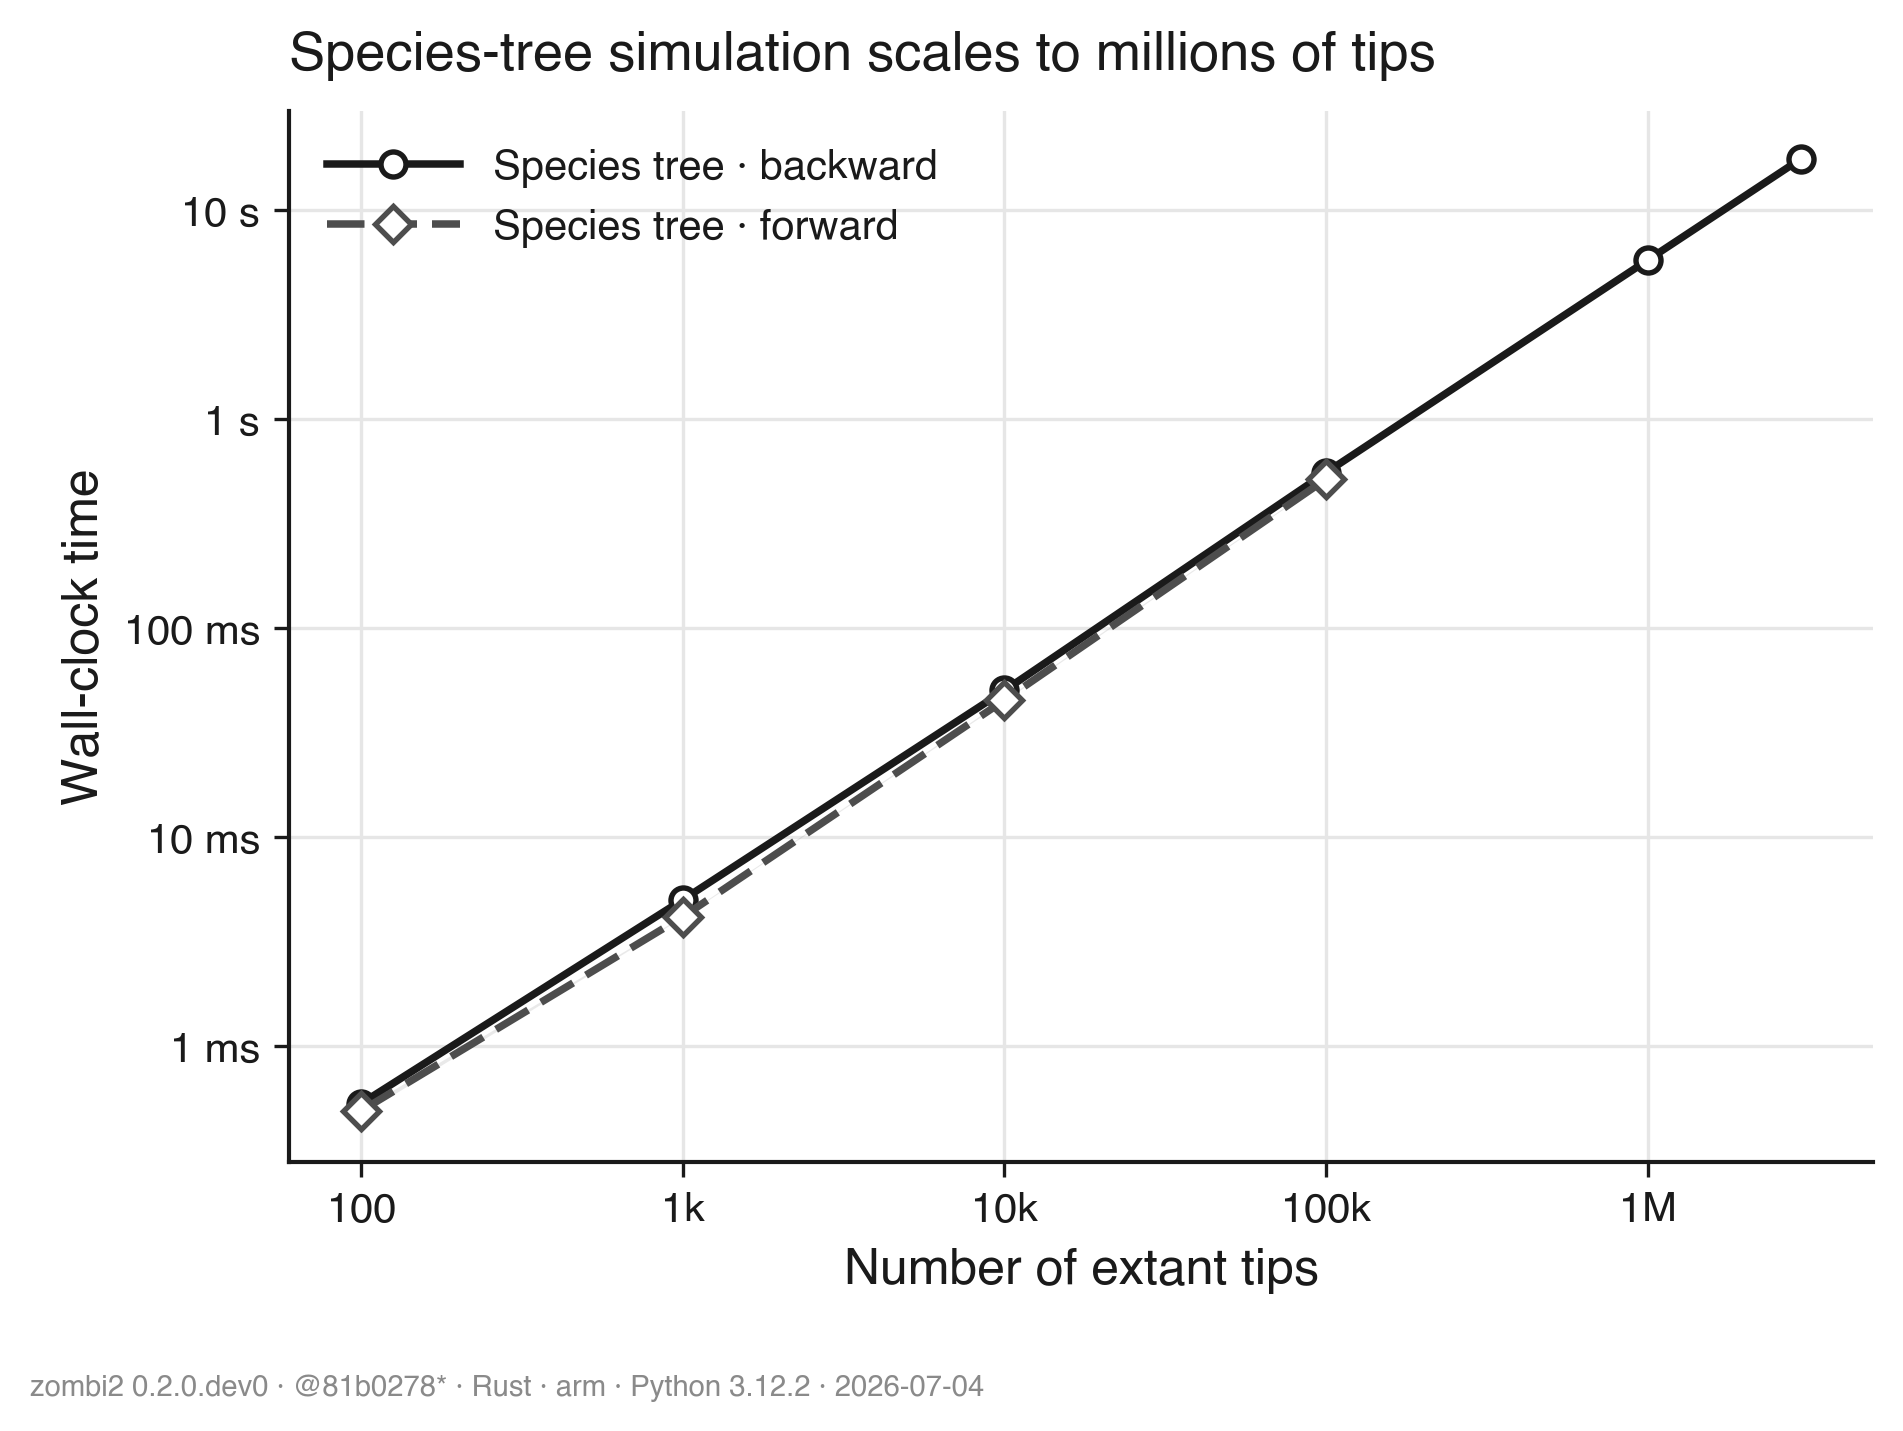
\includegraphics[width=0.82\linewidth]{species_tree_scaling.png}
  \caption{Wall-clock time to simulate a species tree versus number of extant
    tips (log--log). Both samplers track the $\propto N$ guide. Median of repeated
    runs; band is the inter-quartile range.}
  \label{fig:tree}
\end{figure}

% --- gene families ----------------------------------------------------------
\section{Gene-family simulation: three output modes}

Evolving D/T/L/O gene families along a fixed tree offers three outputs of
increasing richness (Figure~\ref{fig:genes}). The \emph{full event log}
(\texttt{output="genomes"}) records every event as a Python object, so its cost
tracks the event count and it is practical to $\sim$\num{100000} tips
(\SI{5.0}{\second}, $\approx$\num{3000000} events). The \emph{event trace}
(\texttt{output="trace"}) keeps the same genealogy as the engine's compact columns
instead of per-event objects --- gene trees remain reconstructable on demand --- so it
runs at roughly twice the counts-only cost yet scales to a million tips
(\SI{2.2}{\second} at \num{100000}, \SI{29}{\second} at \num{1000000}). The
\emph{counts-only} profile (\texttt{output="profiles"}) --- the presence/absence
dataset used for approximate Bayesian computation and downstream analyses --- is the
cheapest and, after the sparse-output change (\S\ref{sec:mem}), scales linearly into
the millions: \SI{66}{\milli\second} at \num{10000} tips, \SI{1.3}{\second} at
\num{100000}, and \SI{18}{\second} at \num{1000000} tips.

\begin{figure}[h]
  \centering
  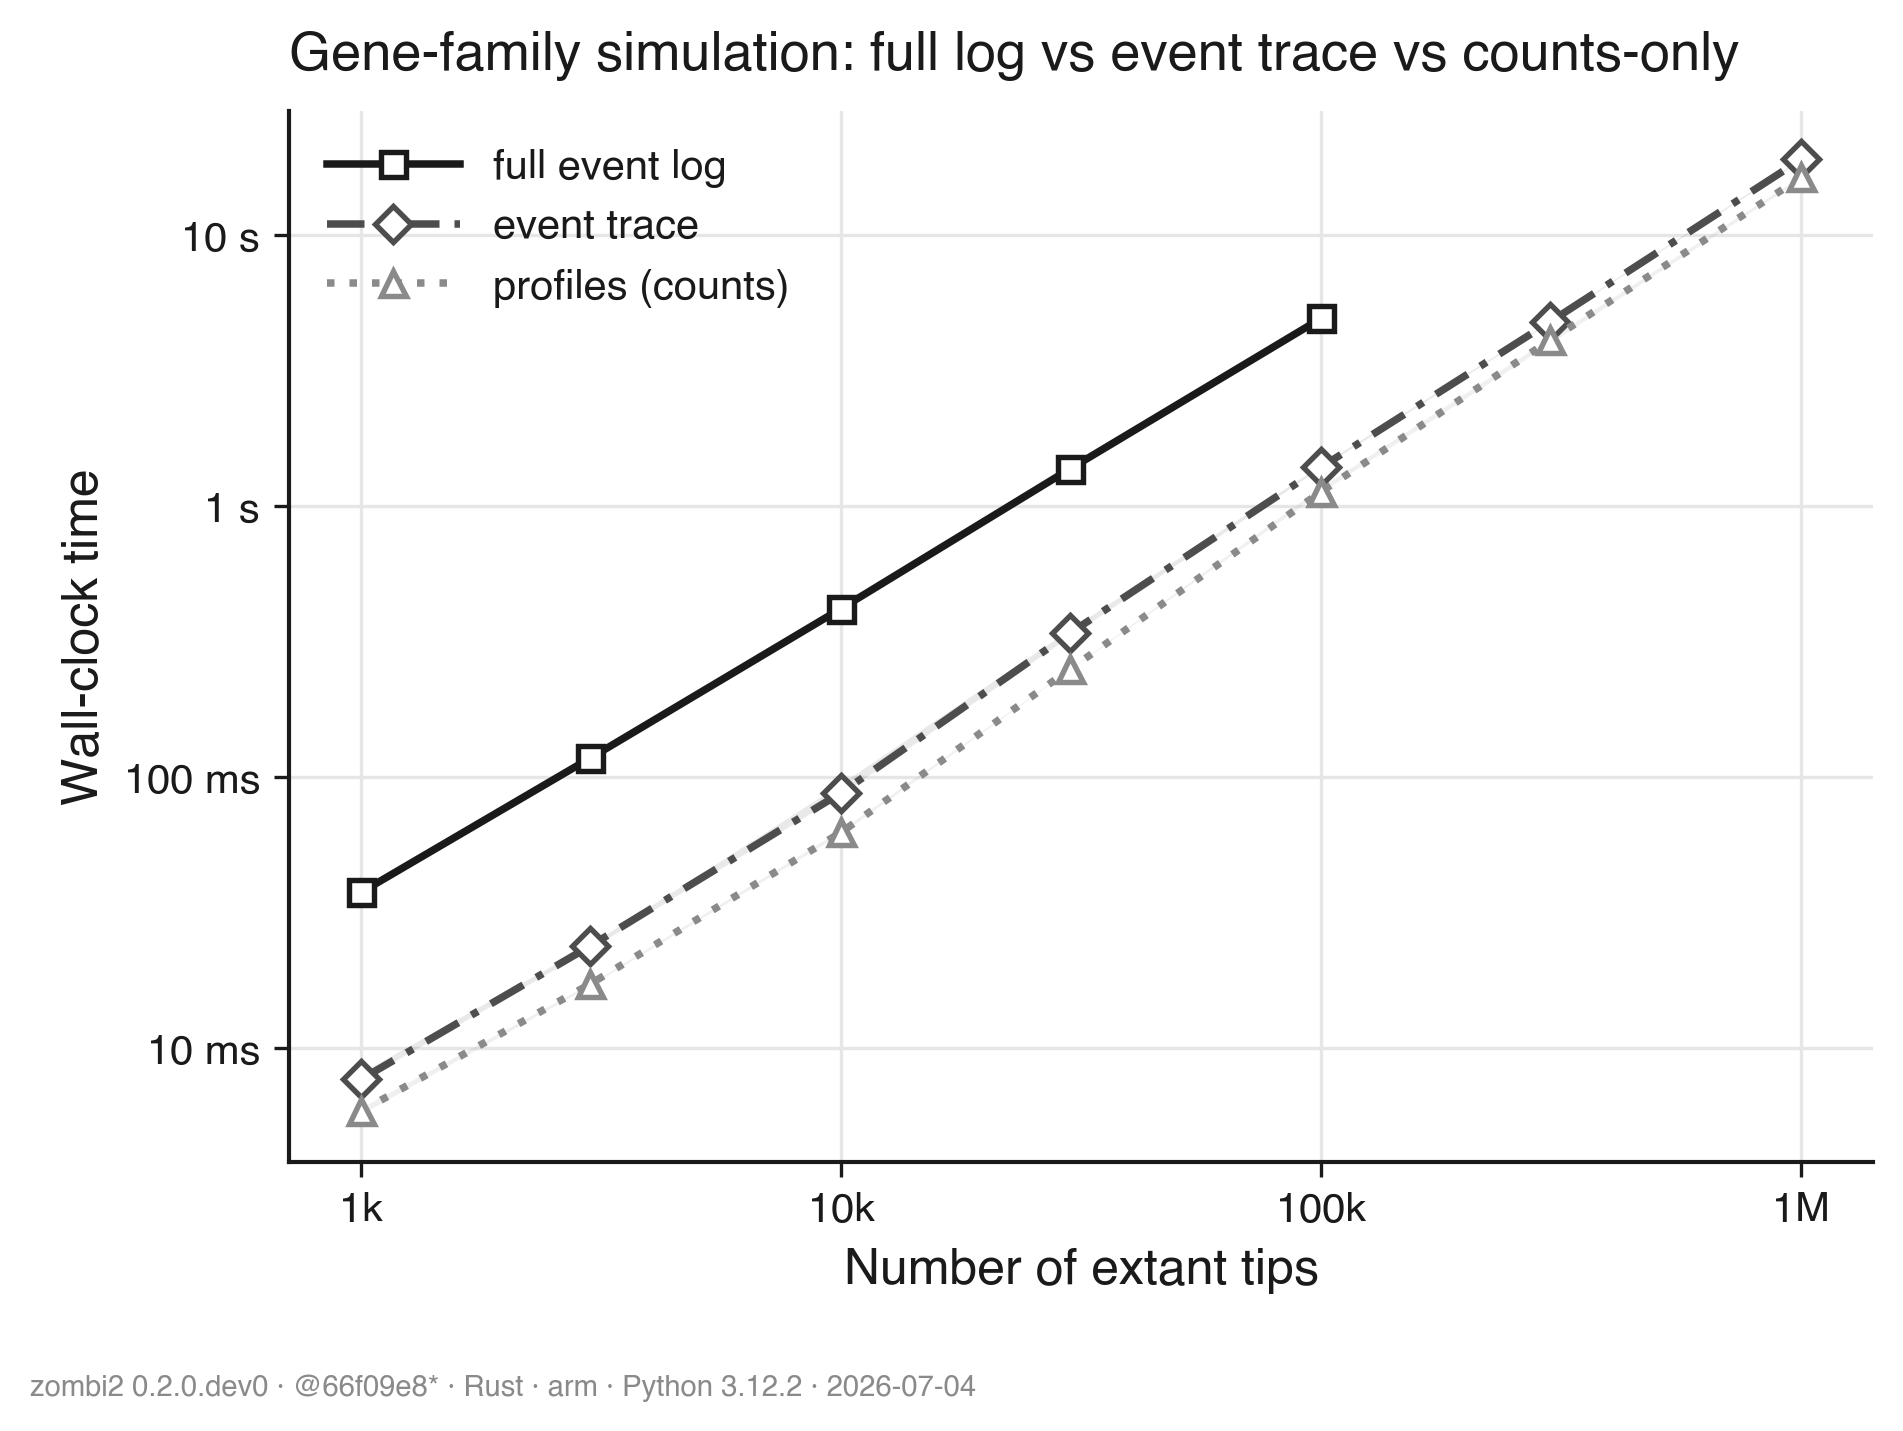
\includegraphics[width=0.82\linewidth]{gene_family_scaling.png}
  \caption{Gene-family simulation versus tip count (log--log). The event trace and
    counts-only profile both run to \num{1000000} tips along the $\propto N$ guide;
    the full event log is heavier and caps near \num{100000} tips.}
  \label{fig:genes}
\end{figure}

% --- memory -----------------------------------------------------------------
\section{Memory footprint and the sparse-output change}
\label{sec:mem}

Peak memory (Figure~\ref{fig:mem}) tells the ``how big can we go'' story. The
species tree is the lightest, roughly \SI{0.7}{GB} per million tips (\SI{0.13}{GB}
at \num{100000}, \SI{0.71}{GB} at \num{1000000}, \SI{2.0}{GB} at \num{3000000}).

The copy-number \emph{profile} was originally a dense
$\text{families}\times\text{species}$ array. Because the number of families grows
in proportion to the number of species, that array is $O(N^2)$ --- it would demand
$\approx$25\,GB of address space already at \num{100000} tips and $\approx$8\,TB at
\num{1000000}, a hard wall well before the simulation itself struggled. We replaced
it with a \textbf{sparse (COO) representation} storing only the present cells, which
is $O(N)$: the profile now costs \SI{0.43}{GB} at \num{100000} tips and
\SI{3.2}{GB} at \num{1000000} --- sizes the dense form could never reach. The
\emph{event trace} sits between the profile and the full log: it holds the whole
event history (as columns, not objects), so it reaches a million tips but at
\SI{11}{GB}, versus the full log's \SI{3.5}{GB} already at \num{100000} tips (one
record per event). Reducing the trace's footprint --- most of it is the
speciation ``carry'' rows, which are redundant given the species tree --- is the
obvious next optimisation.

\begin{figure}[h]
  \centering
  
\includegraphics[width=0.82\linewidth]{memory_scaling.png}
  \caption{Peak resident memory versus tip count (isolated subprocess per size).
    The species tree and the sparse profiles scale linearly into the millions; the
    event trace reaches a million tips at a higher constant; the full event log is
    the memory-heaviest path and caps near \num{100000} tips.}
  \label{fig:mem}
\end{figure}

% --- parallel ---------------------------------------------------------------
\section{Replicate-level parallelism}

Independent replicates are embarrassingly parallel. Running \num{20} independent
full simulations of \num{10000}-tip trees through a process pool
(Figure~\ref{fig:par}) drops the wall-clock from \SI{21.4}{\second} on one worker
to \SI{5.4}{\second} on ten --- a $3.9\times$ speed-up. The curve bends away from
the ideal beyond four workers: this chip has only four performance cores (the
other six are slower efficiency cores), and on macOS each worker re-imports the
library under the \texttt{spawn} start method. On a homogeneous, \texttt{fork}-based
cluster (e.g.\ Linux/SLURM) the same workload scales closer to ideal.

\begin{figure}[h]
  \centering
  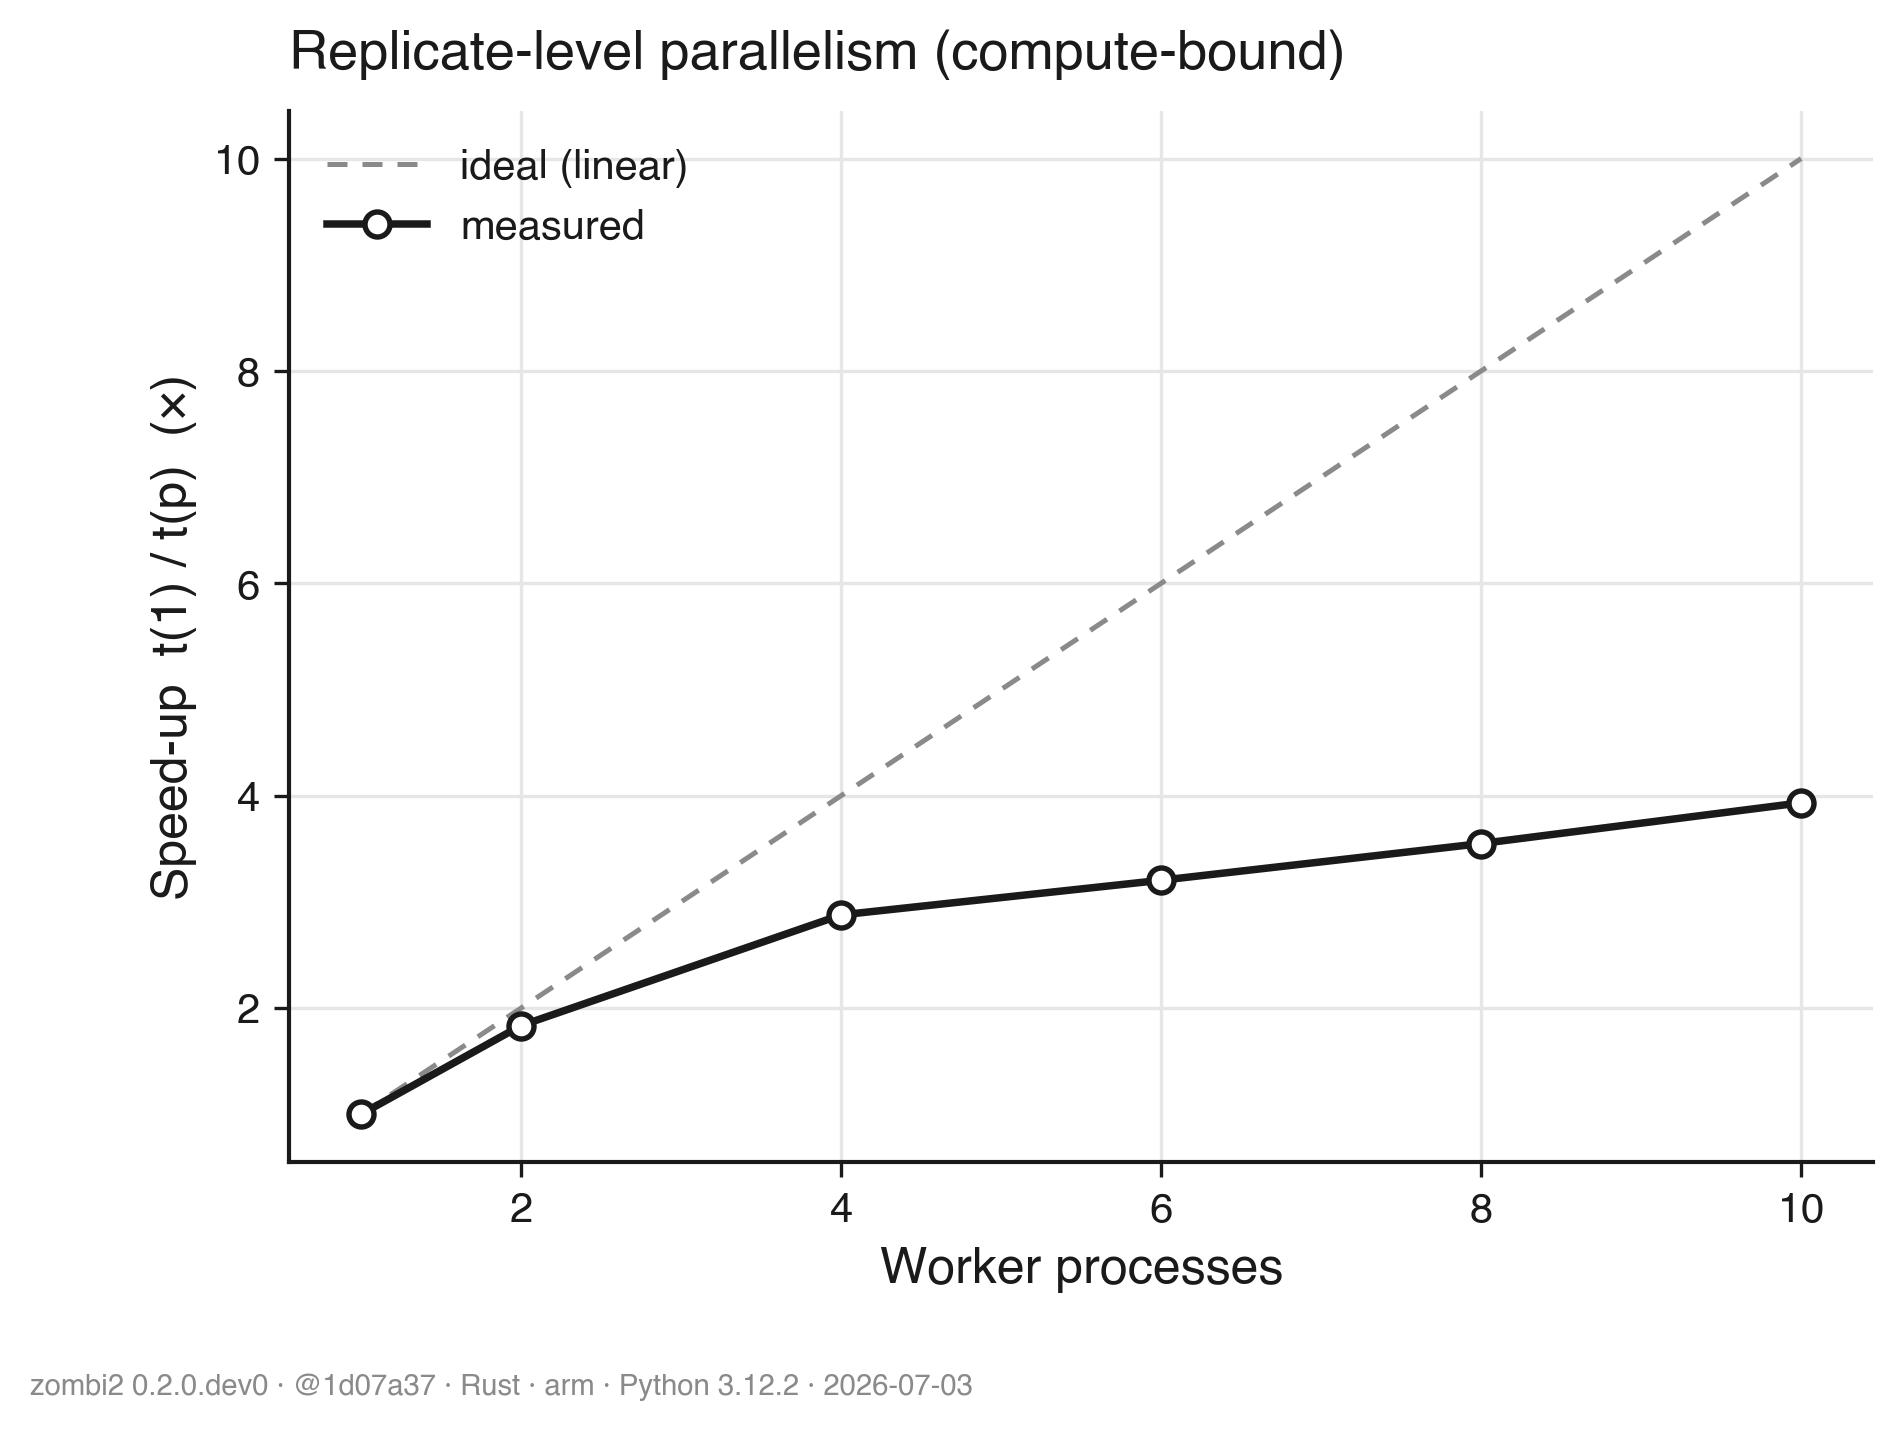
\includegraphics[width=0.82\linewidth]{parallel_scaling.png}
  \caption{Speed-up of a fixed batch of independent simulations versus worker
    processes, against the ideal-linear reference. The plateau past four workers
    reflects the 4-performance/6-efficiency-core split and \texttt{spawn} overhead.}
  \label{fig:par}
\end{figure}

% --- vs ZOMBI 1 -------------------------------------------------------------
\section{Comparison with ZOMBI 1}
\label{sec:vs}

To place the Rust engine in context we ran the \emph{same} gene-family task on the
legacy ZOMBI~1 (pure Python): a pure-birth Yule tree ($\lambda{=}1$) grown to a
matched extant-tip count, the same rate regime ($D{=}0.2$, $T{=}0.1$, $L{=}0.25$,
$O{=}0.5$; \num{20} founding families; size-neutral replacement transfers), timing
only the genome step (ZOMBI~1's \texttt{Gm} mode) in both. The two tools produce
comparable family counts, confirming a like-for-like workload
(Figure~\ref{fig:vs}). ZOMBI~1 is strongly super-linear and reaches a
\textbf{practical ceiling near \num{1200} tips} ($\approx$\SI{55}{\second}); ZOMBI2
runs the same \num{1000}-tip simulation in \SI{38}{\milli\second} versus ZOMBI~1's
\SI{48.2}{\second} --- \headline{over $1000\times$ faster} --- and continues smoothly
to \num{100000} tips and beyond, where ZOMBI~1 is long since infeasible.

\begin{figure}[h]
  \centering
  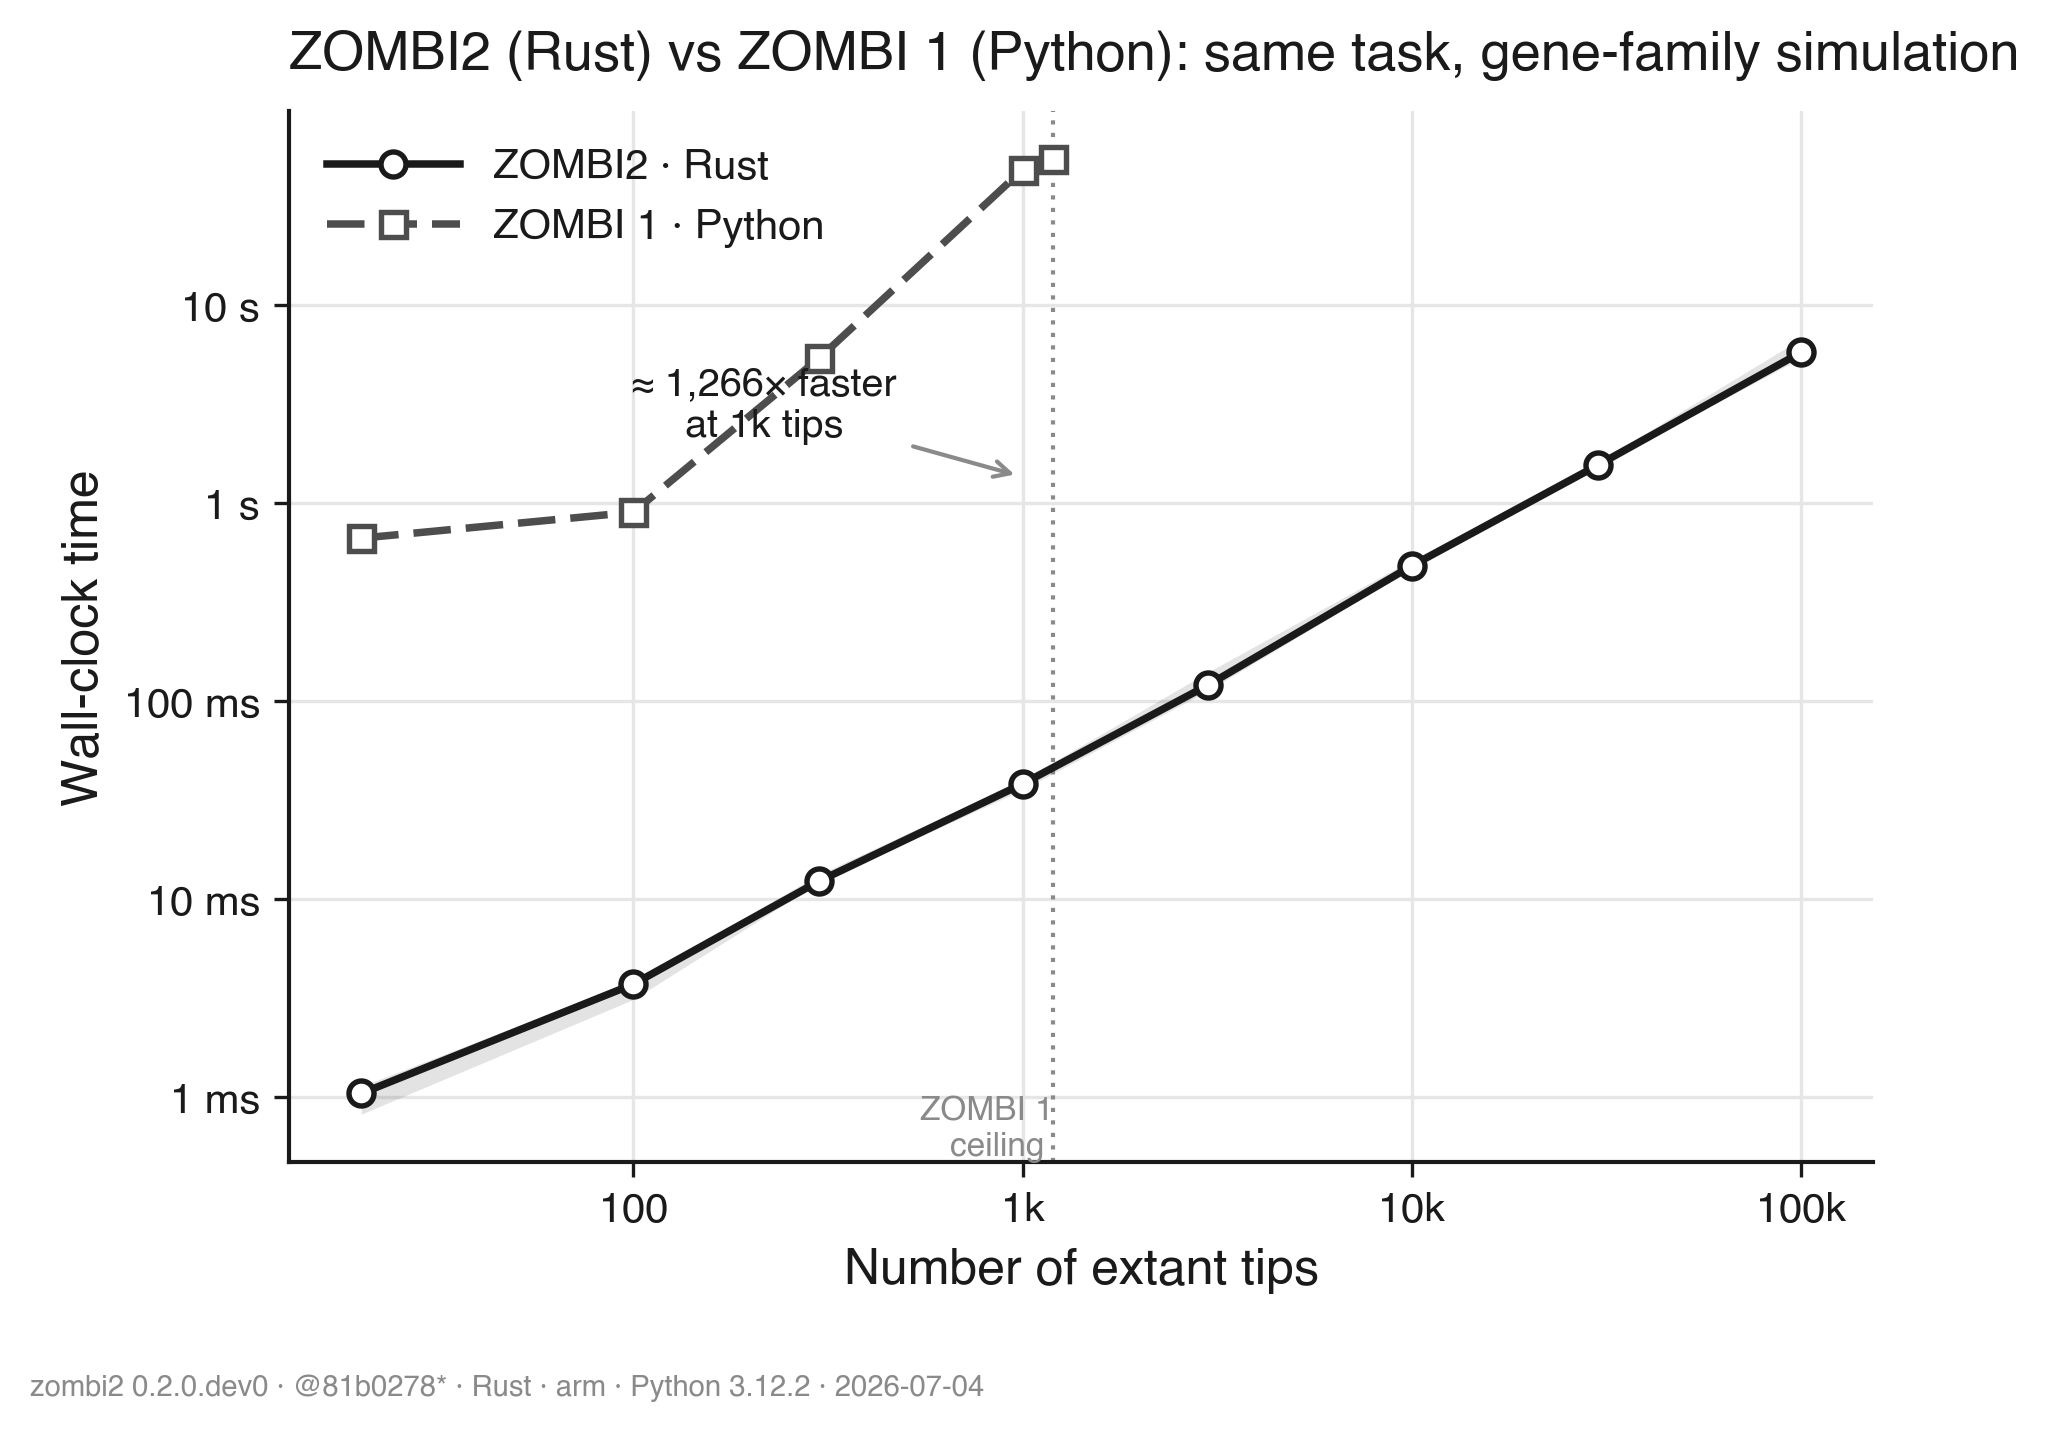
\includegraphics[width=0.72\linewidth]{vs_zombi1.png}
  \caption{ZOMBI2 (Rust) versus ZOMBI~1 (legacy Python) on the same gene-family
    task, matched tip count and rate regime (log--log). ZOMBI2 is over three orders
    of magnitude faster; the dotted line marks ZOMBI~1's practical ceiling.
    Opt-in benchmark (\texttt{vs\_zombi1}); see \texttt{vs\_zombi1/NOTES.md}.}
  \label{fig:vs}
\end{figure}

% --- summary table ----------------------------------------------------------
\section{Summary}

\begin{table}[h]
  \centering
  \caption{Headline results at representative scales (median wall-clock; peak RSS
    from the isolated-subprocess memory runs).}
  \label{tab:summary}
  \small
  \begin{tabular}{l S[table-format=7.0] S[table-format=5.1] l l}
    \toprule
    Task & {Tips $N$} & {Time} & {Unit} & Peak memory \\
    \midrule
    Species tree (backward)   & 1000000 & 5.7  & s & \SI{0.71}{GB} \\
    Species tree (backward)   & 3000000 & 17.6 & s & \SI{2.0}{GB}  \\
    Gene families, full log   & 100000  & 5.0  & s & \SI{3.5}{GB}  \\
    Gene families, event trace& 100000  & 2.2  & s & \SI{1.5}{GB}  \\
    Gene families, event trace& 1000000 & 29.3 & s & \SI{11}{GB}   \\
    Gene families, profiles   & 1000000 & 18.0 & s & \SI{3.2}{GB}  \\
    \bottomrule
  \end{tabular}
\end{table}

\textbf{Bottom line.} Both core operations are linear in tip count and run at
million-tip scale on a laptop; the species tree reaches the millions with room to
spare. The only super-linear component was the dense profile output, now sparse and
linear. Of the three gene-family outputs, the counts-only profile is the one to use
at pure scale, the event trace is the intermediate that keeps gene trees
reconstructable while still reaching a million tips, and the full per-event log --- the
richest but heaviest --- is best kept to $\sim$\num{100000} tips. Against the legacy
ZOMBI~1 the Rust engine is over three orders of magnitude faster on the same task
(\S\ref{sec:vs}). An overview of the headline results is shown in
Figure~\ref{fig:overview}.

\begin{figure}[h]
  \centering
  
\includegraphics[width=\linewidth]{overview.png}
  \caption{Overview: (a) species-tree scaling, (b) the three gene-family output
    modes, (c) ZOMBI2 versus the legacy ZOMBI~1 on the same task.}
  \label{fig:overview}
\end{figure}

\vfill
{\small\color{muted}
Reproducible from \texttt{performance\_analysis/}: \texttt{python run.py} writes raw
timings to \texttt{results/*.json}; \texttt{python plot.py} renders the figures.
Each result file embeds its own provenance (git commit, interpreter, CPU).}

\end{document}
